\documentclass[10pt]{article}



\usepackage{amsmath}
\usepackage{amssymb}
\usepackage{amsthm}
\usepackage{array}
\usepackage{babelbib}
\usepackage{braket}
\usepackage{caption}
\usepackage{colortbl}
\usepackage{rotating}
\usepackage[table]{xcolor}
\usepackage{color}
\usepackage{enumerate}
\usepackage{esint}
\usepackage{eso-pic}
\usepackage{listings}
\usepackage{lscape}
\usepackage{mathtools}
\usepackage{multicol}
\usepackage{multirow}
\usepackage{siunitx}
\usepackage{subcaption}
\usepackage{subdepth}
\usepackage{tcolorbox}
\usepackage{tikz}
\usepackage{titlesec}
\usepackage{titling}
\usepackage{upgreek}
\usepackage{url}
\usepackage{verbatim}
\usepackage{vwcol}
\usepackage{wallpaper}
\usepackage{xfrac}
\usepackage{physics}
\AtBeginDocument{\RenewCommandCopy\qty\SI}
\usepackage[c]{esvect}
\usepackage[utf8]{inputenc}
\usepackage[fleqn]{nccmath}
\usepackage[thicklines]{cancel}
\usepackage[margin=2cm]{geometry}
\usepackage[colorlinks=true,spanish]{hyperref}
\usepackage[oldvoltagedirection]{circuitikz}
\usepackage[greek,spanish,es-tabla,es-nodecimaldot,es-noindentfirst]{babel}
\usepackage[symbol]{footmisc}
\renewcommand{\thefootnote}{\fnsymbol{footnote}}

\sisetup{
  per-mode = fraction,
  inline-per-mode = power,
  detect-all,
  exponent-product = \cdot
}
\hypersetup{
  citecolor = blue,
  linkcolor = blue,
  urlcolor = blue,
  pdfauthor = {Javier Rodrigo López}
}
\captionsetup[figure]{labelfont={bf},name={Figura},labelsep=period}
\captionsetup[table]{labelfont={bf},name={Tabla},labelsep=period}
\titleformat{\section}{\normalfont\Large\bfseries}{\thesection}{1em}{}[{\titlerule[0.8pt]}]
\titleformat{\subsubsection}{\normalfont\normalsize\bfseries}{\thesubsubsection}{1em}{}[{}]
\titlespacing{\section}{0pt}{2\parskip}{\parskip}
\titlespacing{\subsection}{0pt}{\parskip}{0pt}
\titlespacing{\subsubsection}{0pt}{\parskip}{0pt}
\usepackage{enumitem}
\setlist{before={\parskip=3pt}, after=\vspace{\baselineskip}}
\setlength{\parindent}{0pt}
\setlength{\parskip}{0.5em}
\renewcommand\thesubsubsection{\arabic{subsubsection}}

\usepackage{booktabs}
\usepackage{bigstrut}

\renewcommand{\vec}{\vv}

% Tipografía
% \renewcommand{\familydefault}{\sfdefault}
% \renewcommand{\rmdefault}{\sfdefault}

% Para escribir decibelios SPL
\DeclareSIUnit\dbspl{dB\ensuremath{_{\textnormal{SPL}}}}
\DeclareSIUnit\dBlin{dB\ensuremath{_{\textnormal{Lin}}}}
\DeclareSIUnit\dBA{dB\ensuremath{_{\textnormal{A}}}}


\title{\Huge Práctica 1.3. Altavoces \\\huge Laboratorio de Sistemas Electroacústicos}
\author{Javier Rodrigo López}
\date{\today}

\begin{document}
\maketitle
% \tableofcontents
\setcounter{subsubsection}{8}

\subsubsection{Adjuntar las gráficas de respuesta del sistema de bass-reflex en campo cercano (diafragma y abertura). Obtener de la gráfica la fase relativa de las dos respuestas (diafragma y abertura) en las siguientes frecuencias: \qty{15}{\hertz }, \qty{40}{\hertz } y \qty{300}{\hertz }. Comentar el resultado.}

\begin{figure}[hbtp]
  \centering
  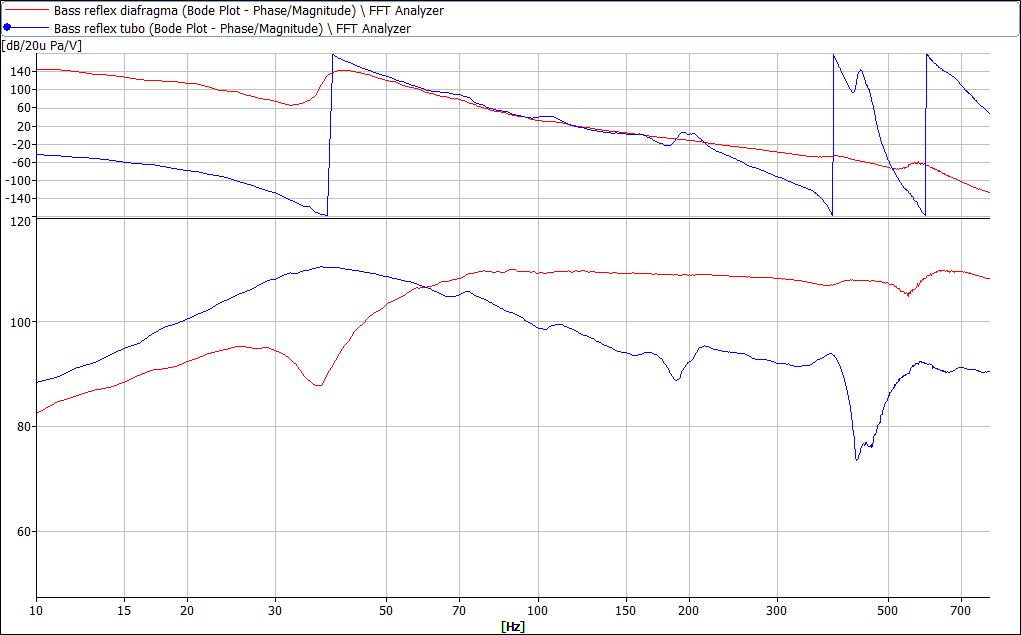
\includegraphics[width=0.8\linewidth]{Imágenes/Diafragma_vs_tubo.png}
  \caption{Respuesta del bass-reflex del diafragma (rojo) y del tubo (azul), ambas medidas en cámara anecoica a una distancia muy corta para evitar contaminación del otro elemento.}
  \label{fig:Diafragma_vs_tubo.png}
\end{figure}

Se obtienen las diferencias de fase en las tres frecuencias especificadas a partir de los datos de la gráfica. El resultado aparece en la \autoref{eq:2}.

\begin{equation} \label{eq:2}
  \Delta \phi = \abs{\phi_{\text{diafragma}} - \phi_{\text{tubo}}} = \begin{cases}
    \ang{187,28} \approx \ang{180} & \text{a }\qty{15}{\hertz }  \\
    \ang{26,96}                    & \text{a }\qty{40}{\hertz }  \\
    \ang{54.46}                    & \text{a }\qty{300}{\hertz }
  \end{cases}
\end{equation}

Estos resultados, que incluyen un indicativo del valor teórico al que se deben aproximar, implican varias cosas. A la frecuencia de \qty{15}{\hertz }, se obtiene un desfase de \ang{187.28}, debido a que se está trabajando a una frecuencia menor a la frecuencia de resonancia del sistema. Esto provoca grandes pérdidas de nivel acústico a bajas frecuencias con respecto al sistema de caja cerrada. A la frecuencia de \qty{40}{\hertz }, se obtiene un desfase de \ang{26.96}, que se acerca bastante a \ang{0}, lo que indica que el sistema está trabajando en una frecuencia cercana a la de sintonía. En este punto lo que debe ocurrir es una suma en fase de ambas señales, la del diafragma y la de la abertura. Por último, a la frecuencia de \qty{300}{\hertz }, se obtiene un desfase de \ang{54.46}. Hasta frecuencias de \qty{200}{\hertz } ambos elementos trabajaban en fase, pero entonces se observa que la diferencia de fase aumenta notablemente con la frecuencia.

\subsubsection{Adjuntar las gráficas de respuesta del sistema de bass-reflex en campo lejano (bass-reflex y caja cerrada). Obtener y representar en Excel (escala de frecuencias logarítmica desde \qty{10}{\hertz }) la función de transferencia anecoica del sistema bass-reflex (Hb) (sólo amplitud) usando la \autoref{eq:1}. Representar en la misma gráfica anterior la función de transferencia anecoica de la caja acústica hermética $H_{c \text{ (caja cerrada)}} (\qty{2}{\centi\metre })$. Estimar las pendientes de subida en dB/oct (método de la recta superpuesta) y determinar la máxima ganancia del bass-reflex respecto a la caja hermética.}

\begin{equation} \label{eq:1}
  H_{b \text{(bass-reflex)}} = \frac{H_{b \text{ (bass-reflex)}}(\qty{2}{\metre })}{H_{c \text{ (caja cerrada)}} (\qty{2}{\metre })} H_{c \text{ (caja cerrada)}} (\qty{2}{\centi\metre })
\end{equation}

En la \autoref{fig:bass-reflex_y_caja_cerrada.png} se aprecia el comportamiento acústico en frecuencia del diafragma y del tubo. Con estos datos es posible entender mejor el funcionamiento del sistema bass-reflex. Para ello conformaremos una sola gráfica donde se pueda comprobar la diferencia con el sistema de caja cerrada. En la \autoref{fig:grafica_excel.png} aparecen representados los dos sistemas. Esta gráfica ha sido obtenida mediante la \autoref{eq:1}. Se estima que la recta trazada abarca verticalmente unos 85 dB (8 cuadrículas y media), y horizontalmente se sabe que se trata de una década. Se trata de una pendiente de aproximadamente 85 dB/década. Para obtener la pendiente en octavas se hace de la siguiente forma:
\begin{align*}
  \frac{10 \log \left( 2f \right) - 10 \log \left( f \right) }{\Delta L} & = \frac{10 \log \left( 10 f \right) - 10 \log \left( f \right) }{85}                              \\
  \Delta L                                                               & =85 \frac{\log \left( 2 \right) }{\log \left( 10 \right)} = 25.6 \approx \qty{24}{\dB\per octava}
\end{align*}

Este resultado es coherente puesto que el sistema de bass-reflex es un sistema de 4º orden. Por otro lado, la recta que se ubicaría sobre la curva naranja (sistema de caja cerrada) tendría una pendiente aproximada de \qty{12}{\dB\per octava}, ya que se trata de un sistema de segundo orden.

\begin{figure}[hbtp]
  \centering
  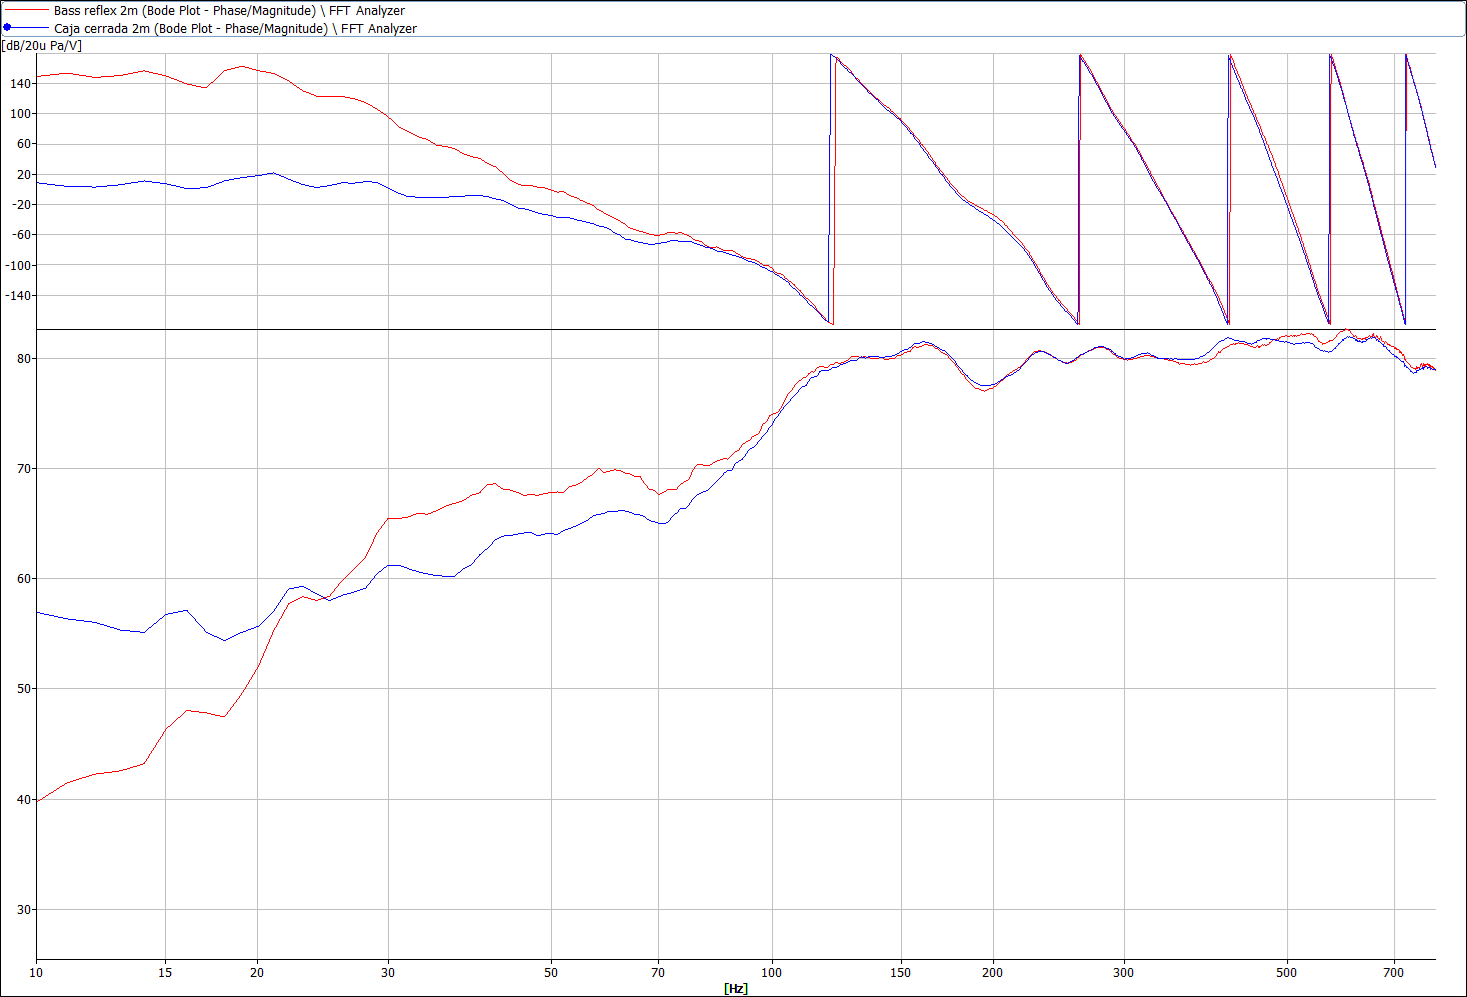
\includegraphics[width=0.8\linewidth]{Imágenes/bass-reflex_y_caja_cerrada.png}
  \caption{Respuesta del sistema bass-reflex (rojo) y de la caja cerrada (azul) en campo lejano (a \qty{2}{\metre }).}
  \label{fig:bass-reflex_y_caja_cerrada.png}
\end{figure}

\begin{figure}[hbtp]
  \centering
  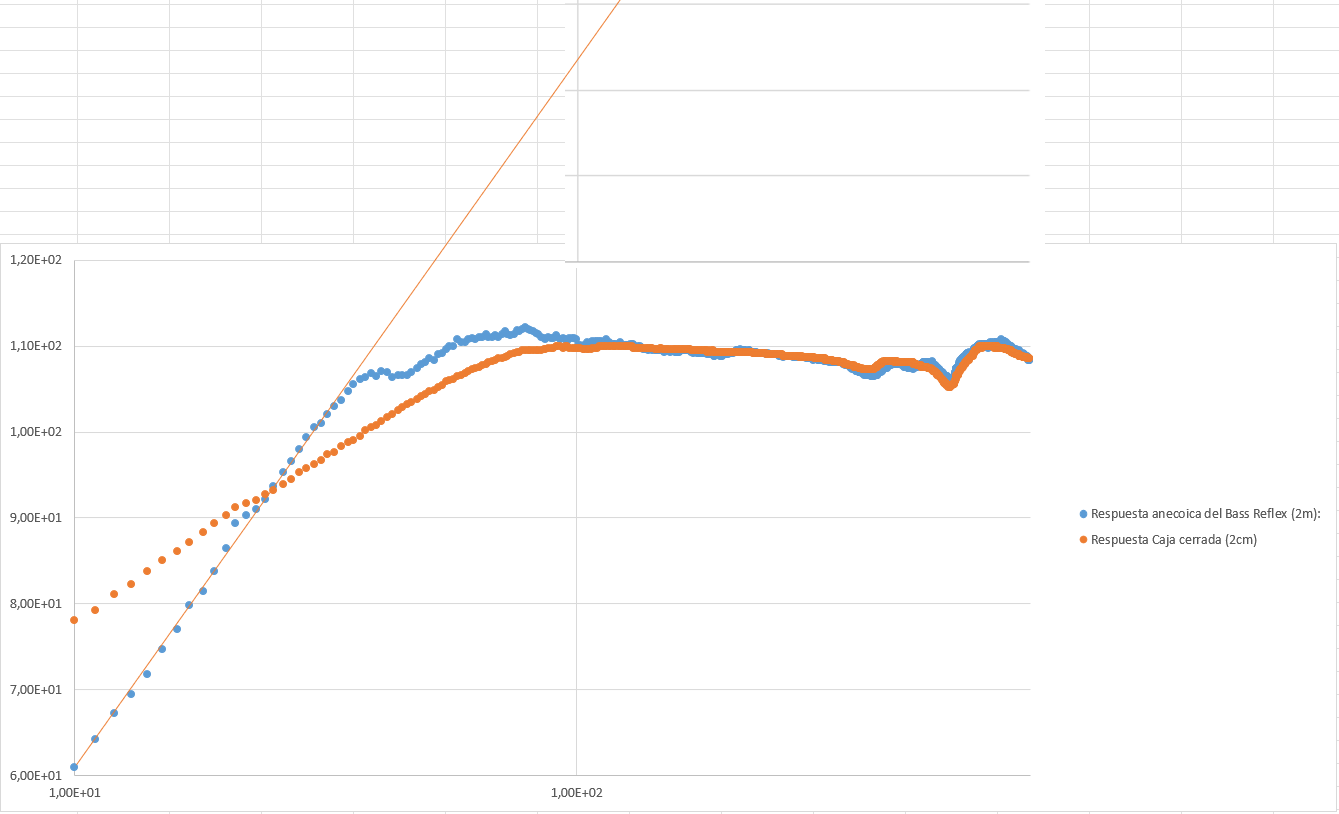
\includegraphics[width=0.8\linewidth]{Imágenes/grafica_excel.png}
  \caption{Método de la recta superpuesta para obtener la pendiente de la función de transferencia del sistema bass-reflex.}
  \label{fig:grafica_excel.png}
\end{figure}

\subsubsection{Adjuntar las gráficas de desplazamiento, velocidad y aceleración del diafragma tanto de la caja hermética como del sistema de bass-reflex. Para pasar de desplazamiento a velocidad y a aceleración aplicar la ponderación $j \omega$ desde el campo ``functions'' de PULSE. Obtener de las gráficas y presentar en forma de tabla los siguientes valores representativos (usar unidades lineales por voltio): $x_{d0c}$, $x_{d0b}$, $u_d (f_c)$, $a_{d0c}$ y $a_{d0b}$.}

Entendiendo que los parámetros que incluyen el 0 en su subíndice se refieren al valor medido en la gráfica a la frecuencia de sintonía, y que la frecuencia $f_c$ en realidad es $f_b$ y se refiere a la frecuencia de sintonía del sistema de bass-reflex, se obtienen los siguientes valores:

\begin{table}[hbtp]
  \centering
  \begin{tabular}{|l|l|l|} \hline
                   & Caja cerrada                                                 & Bass-reflex                                                  \\ \hline
    Desplazamiento & $x_{d0c} = \qty{164.7}{\micro\metre\per\volt}$               & $x_{d0b} = \qty{36.4}{\micro\metre\per\volt}$                \\ \hline
    Velocidad      & $u_{dc}(f_c) = \qty{41.4}{\milli\metre\per\second\per\volt}$ & $u_{db}(f_c) = \qty{9.15}{\milli\metre\per\second\per\volt}$ \\ \hline
    Aceleración    & $a_{d0c} = \qty{10.41}{\metre\per\second\squared\per\volt}$  & $a_{d0b} = \qty{2.3}{\metre\per\second\squared\per\volt}$    \\ \hline
  \end{tabular}
\end{table}

\begin{figure}[htp]
  \centering
  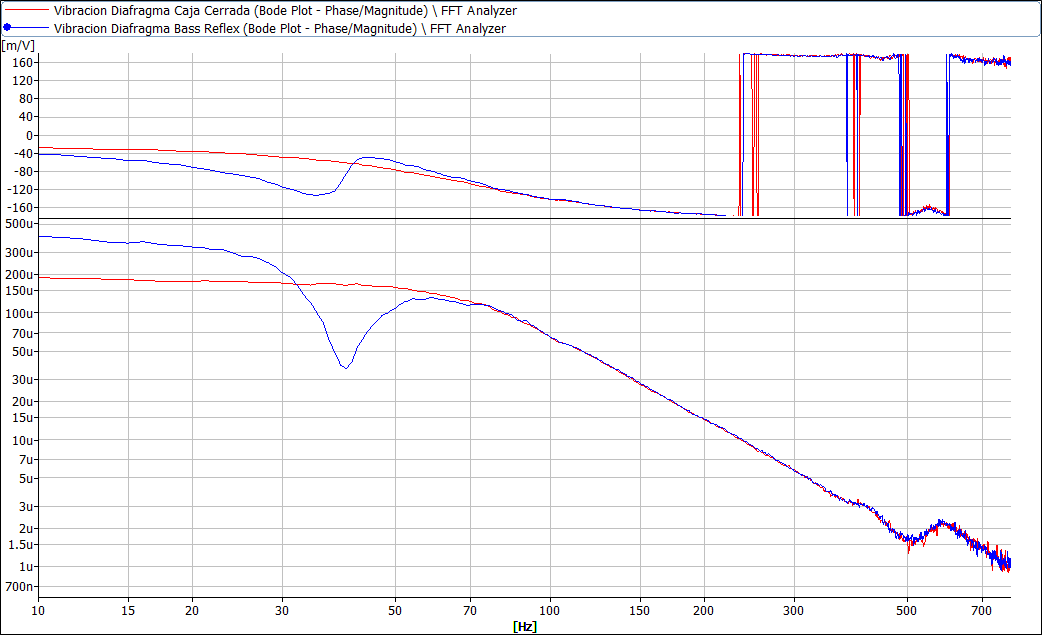
\includegraphics[width=0.8\linewidth]{Imágenes/Desplazamiento.png}
  \caption{Desplazamiento del diafragma en caja cerrada (rojo) y en bass-reflex (azul).}
  \label{fig:Desplazamiento.png}
\end{figure}
\begin{figure}[htp]
  \centering
  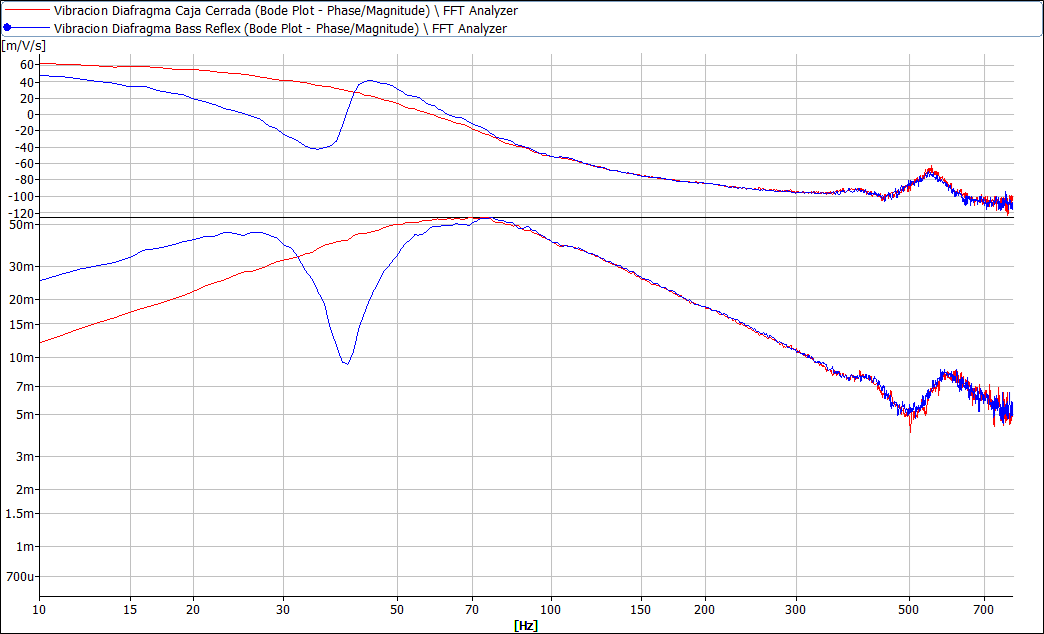
\includegraphics[width=0.8\linewidth]{Imágenes/Velocidad.png}
  \caption{Velocidad del diafragma en caja cerrada (rojo) y en bass-reflex (azul).}
  \label{fig:Velocidad.png}
\end{figure}
\begin{figure}[htp]
  \centering
  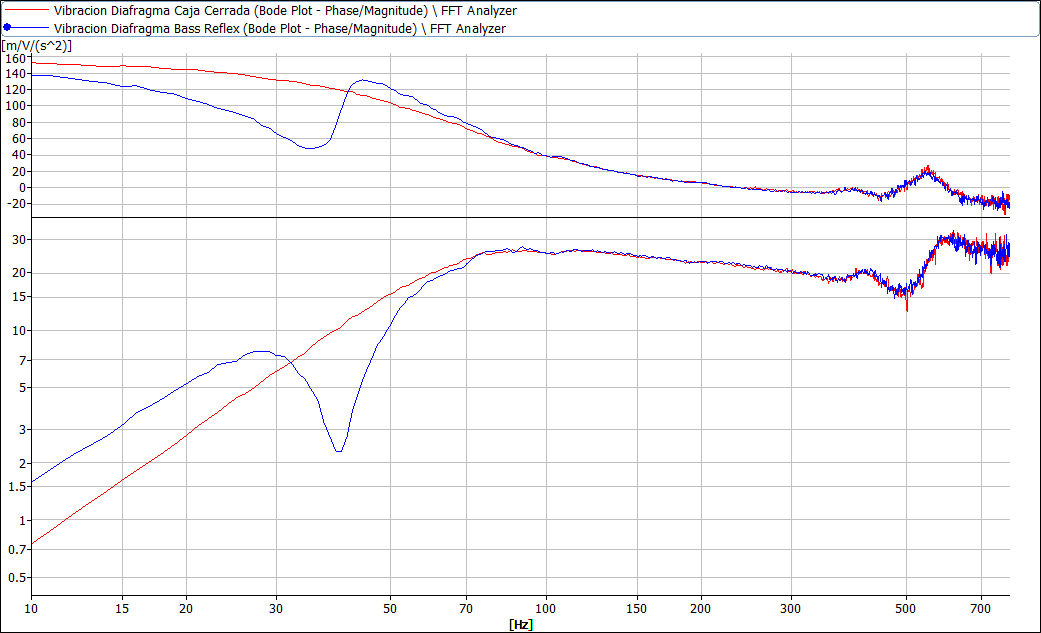
\includegraphics[width=0.8\linewidth]{Imágenes/Aceleración.png}
  \caption{Aceleración del diafragma en caja cerrada (rojo) y en bass-reflex (azul).}
  \label{fig:Aceleracion.png}
\end{figure}

\subsubsection{Adjuntar la gráfica de impedancia del sistema del sistema de bass-reflex (en Moodle se proporcionan estas curvas para la caja abierta, sin tubo añadido). Determinar las frecuencias características a partir de los cruces por cero de la fase y comprobar la correspondencia de estas frecuencias con otras obtenidas durante la práctica (consultar la teoría).}

En las figuras \ref{fig:Zee_Woofer_en_caja_hermetica.png}, \ref{fig:Zee_Woofer_en_caja_con_filtros.png}, \ref{fig:Zee_Woofer_en_sistema_bass_reflex.png} se puede observar la impedancia eléctrica de entrada $Z_{ee}$ para cada uno de los tres sistemas estudiados. Aquellas frecuencias a las que se produce un cruce por cero de la fase pueden ser frecuencias significativas.

\begin{figure}[hbtp]
  \centering
  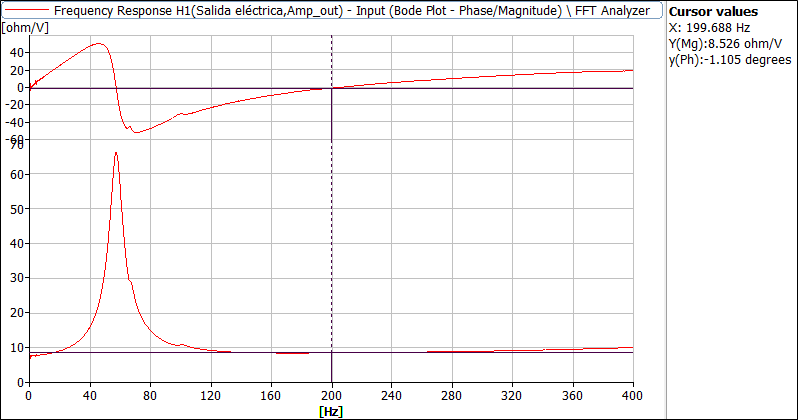
\includegraphics[width=0.8\linewidth]{Imágenes/Zee_Woofer_en_caja_hermetica.png}
  \caption{Impedancia eléctrica de entrada de la caja hermética.}
  \label{fig:Zee_Woofer_en_caja_hermetica.png}
\end{figure}

\begin{figure}[hbtp]
  \centering
  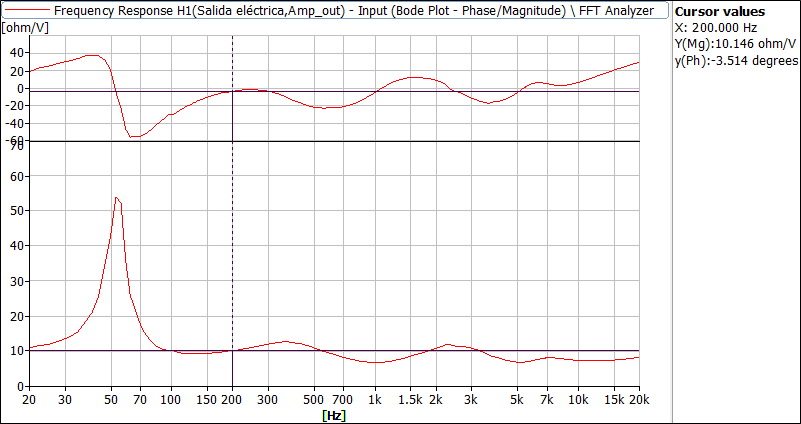
\includegraphics[width=0.8\linewidth]{Imágenes/Zee_Woofer_en_caja_con_filtros.png}
  \caption{Impedancia eléctrica de entrada de la caja en conjunto con los filtros de cruce}
  \label{fig:Zee_Woofer_en_caja_con_filtros.png}
\end{figure}

\begin{figure}[hbtp]
  \centering
  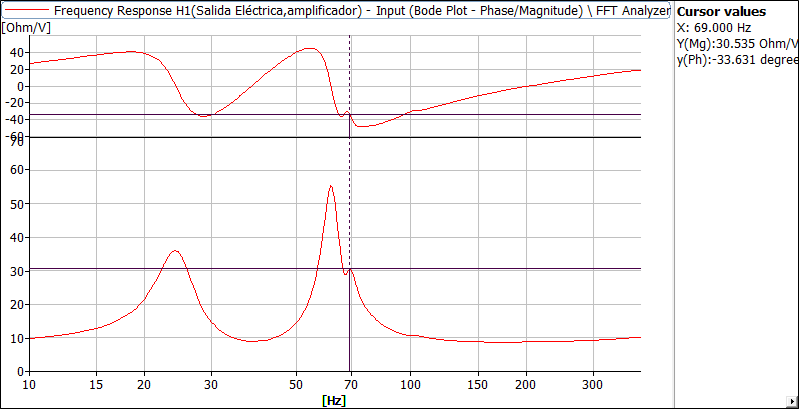
\includegraphics[width=0.8\linewidth]{Imágenes/Zee_Woofer_en_sistema_bass_reflex.png}
  \caption{Impedancia eléctrica de entrada del sistema bass-reflex.}
  \label{fig:Zee_Woofer_en_sistema_bass_reflex.png}
\end{figure}

\end{document}
